%\begin{description}

%\vspace{1ex} 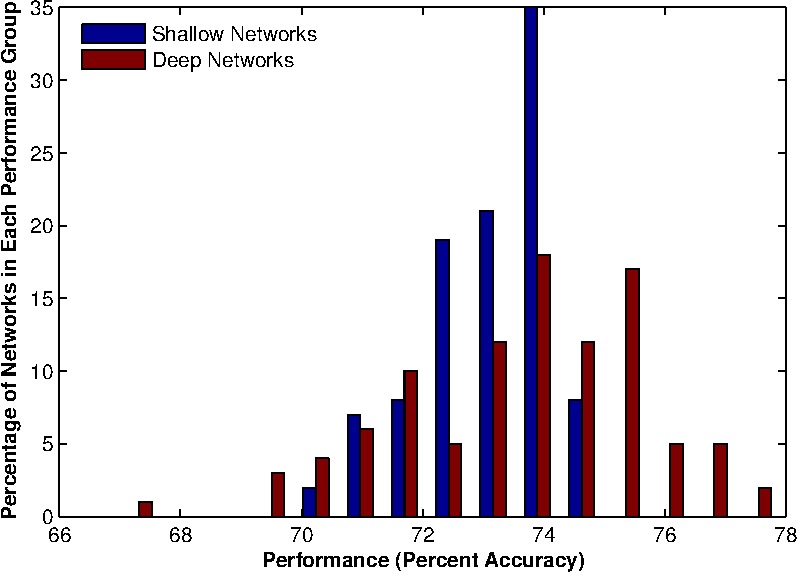
\includegraphics[width=0.7\textwidth]{Figs/e_fig7s-crop.pdf}\\
%{\bf Figure \SFpef. Performance of shallow and deep networks.}
%
%\vspace{2ex} 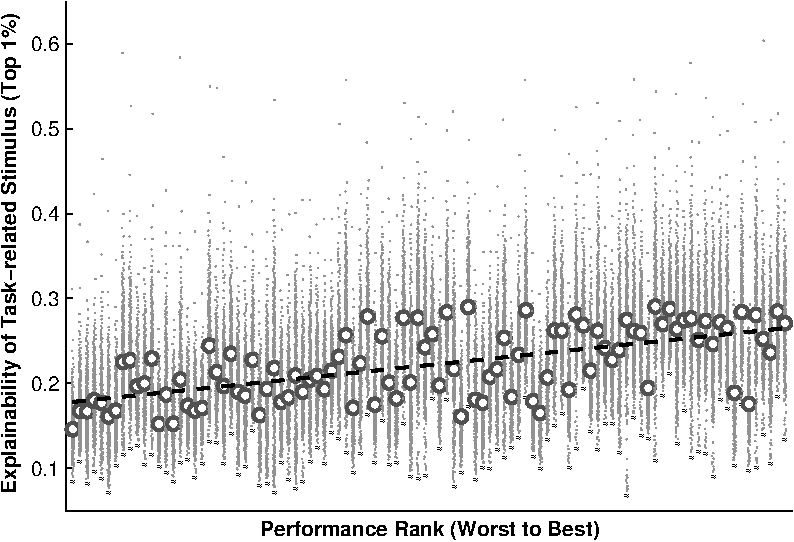
\includegraphics[width=0.7\textwidth]{Figs/e_fig4b.pdf}\\
%{\bf Figure \SFexp. Explanation power vs.~performance rank.} $P < 0.001$. %Enter optional descriptive information here.
%
%\vspace{2ex} 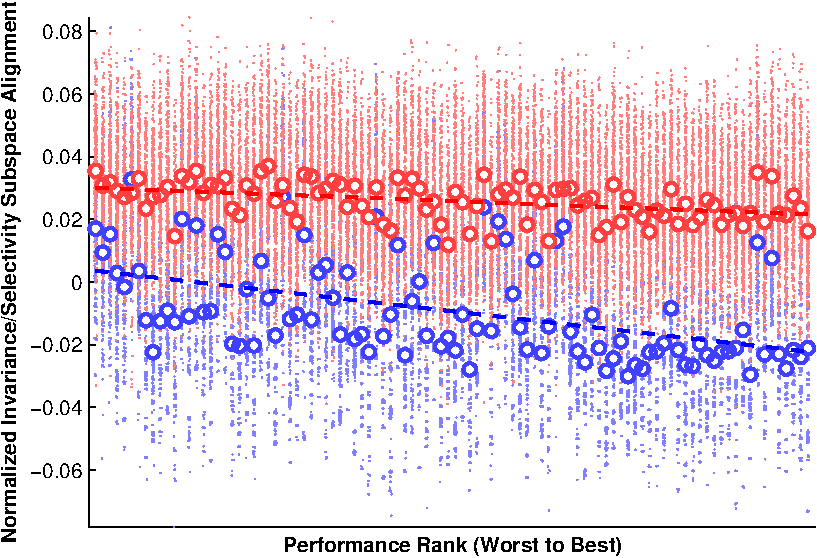
\includegraphics[width=0.7\textwidth]{Figs/e_fig5d.pdf}\\
%{\bf Figure \SFaln. Invariance and selectivity subspace alignment vs.~performance rank.} Both $P < 0.001$.
%
%\vspace{2ex} 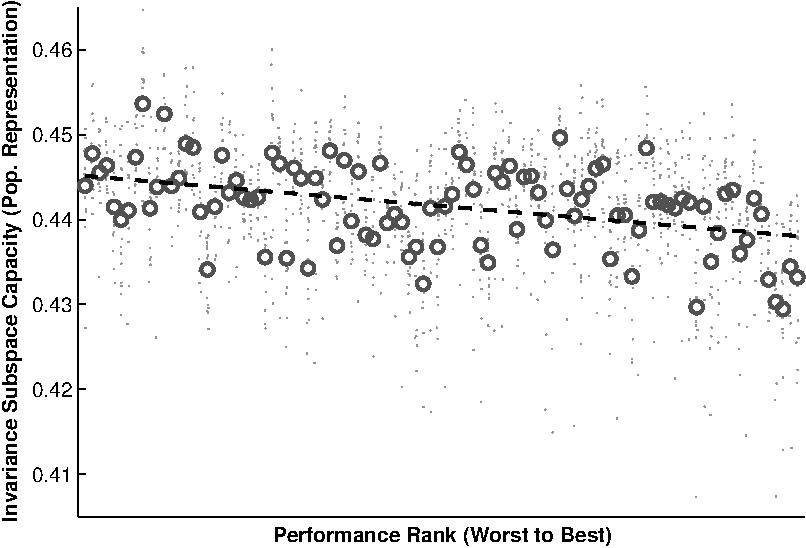
\includegraphics[width=0.7\textwidth]{Figs/e_fig5b.pdf}\\
%{\bf Figure \SFinc. Invariance subspace capacity vs.~performance rank.} $P < 0.001$.
%
%\vspace{2ex} 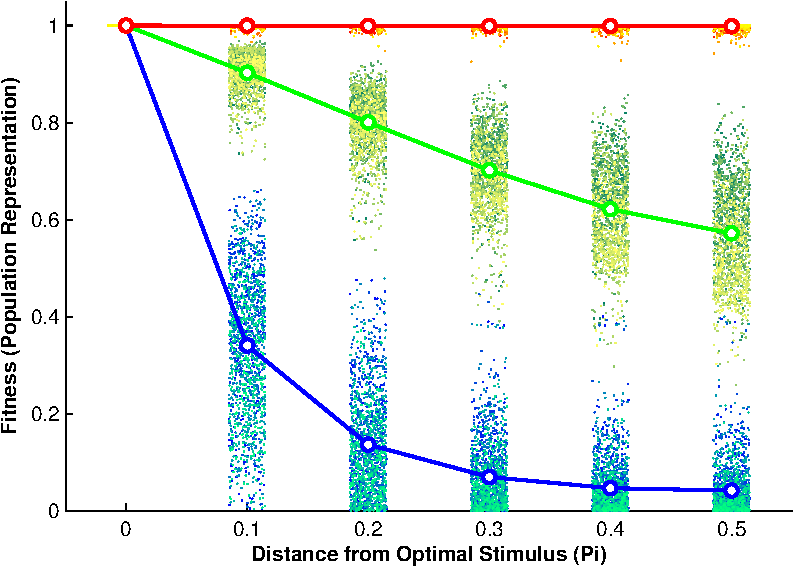
\includegraphics[width=0.7\textwidth]{Figs/e_fig5a.pdf}\\
%{\bf Figure \SFfda. Fitness-distance diagram.} $P$ value? %Corr of Random Walk, Multi Corr after adding that? why r is low? kernel selection.
%
%\vspace{2ex} 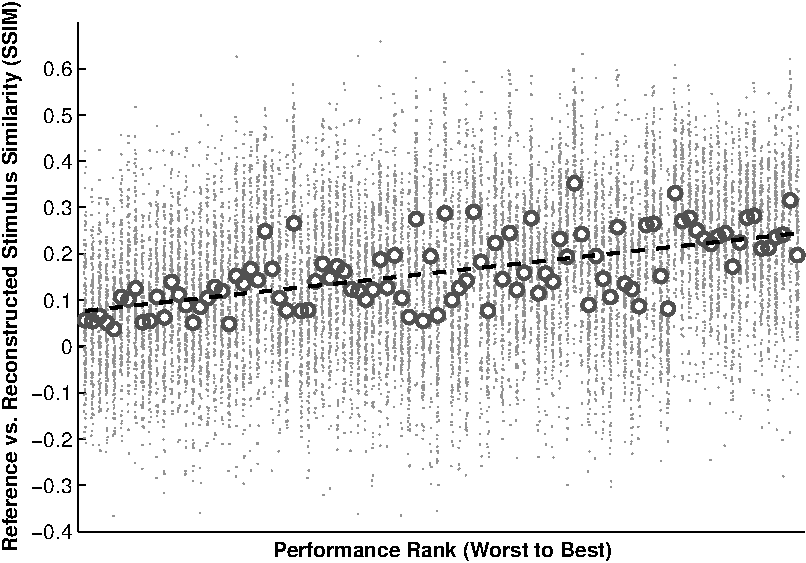
\includegraphics[width=0.7\textwidth]{Figs/e_fig6b.pdf}\\
%{\bf Figure \SFenc. Encoding specificity vs.~performance rank.} $P < 0.001$.

%\item{\bf Figure S0. All OS.}
%\item\bf Figure S6. All corr plot.} PARTIAL correlation!?
%\item{\bf Text S1. LFW EXP DETAILS (FT DIM, SVM SETTING)} retinotopic. %latex textblock?
%\item{\bf Text S2. Details of numerical optimzation (invariance subspace; encoding specificity).} %enc spc: regularized and more structural, especially important for highly noise tolerant networks; multi-resolution
% $\lambda\left\|\nabla^{2}x\right\|_{F}$

%\item{\bf Text S1. Details of numerical optimization (invariance subspace; encoding specificity).}
%\item enc spc: regularized and more structural, especially important for highly noise tolerant networks; multi-resolution

%\end{description}

\newcommand{\beginsupplement}{\setcounter{figure}{0} \renewcommand{\thefigure}{S\arabic{figure}}}
\beginsupplement

\begin{figure}[H]
\centering 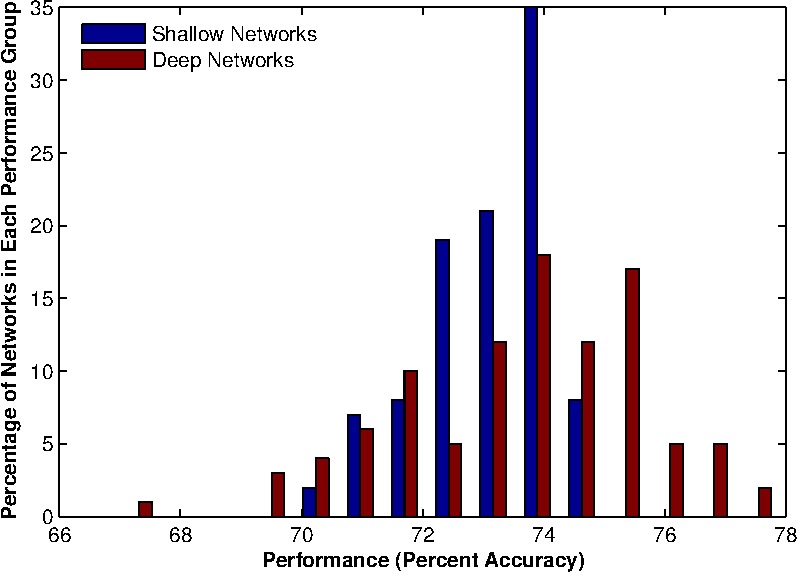
\includegraphics[width=0.6\textwidth]{Figs/e_fig7s-crop.pdf} 
\caption{ 
{\bf Distributions of shallow and deep network performances.} Performances of the randomly generated 100 shallow and 100 deep networks are obtained via 10-fold cross validations of 6,000 face image pairs. Feature vectors used in the linear SVM classifier are generated via sliding the receptive fileds throughout entire images and concatenating the population representations (as defined in convolutional neural networks). Maximum and mean of performances of the deep networks are both significantly higher than those of the shallow networks (with permutation tests, $p<0.001$ and $p=0.008$ respectively). See \cite{cox2011beyond} for more details.}
\label{fig:SFpef}
\end{figure}

\begin{figure}[H]
\centering 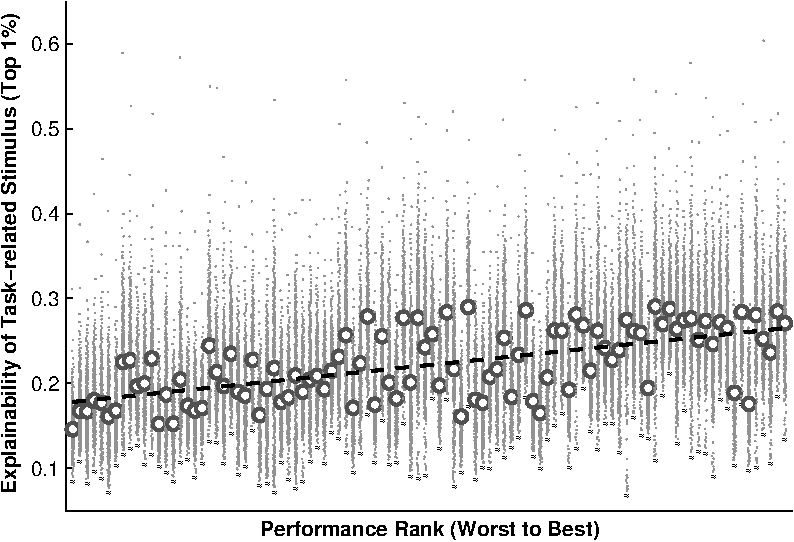
\includegraphics[width=0.6\textwidth]{Figs/e_fig4b.pdf} 
\caption{ 
{\bf Explanation power vs.~performances of deep networks.} Each distribution from left to right shows the top 1\% explainabilities of the task-related stimuli within each of the 32 top-layer unit representations of a deep network. Performance ranks, instead of performance values, are used for visualization purposes. Means of distributions are plotted as gray circles and the linear regression as dashed black line. Significance of slope using permutation test has $p < 0.001$.}
\label{fig:SFexp}
\end{figure}

\begin{figure}[H]
\centering 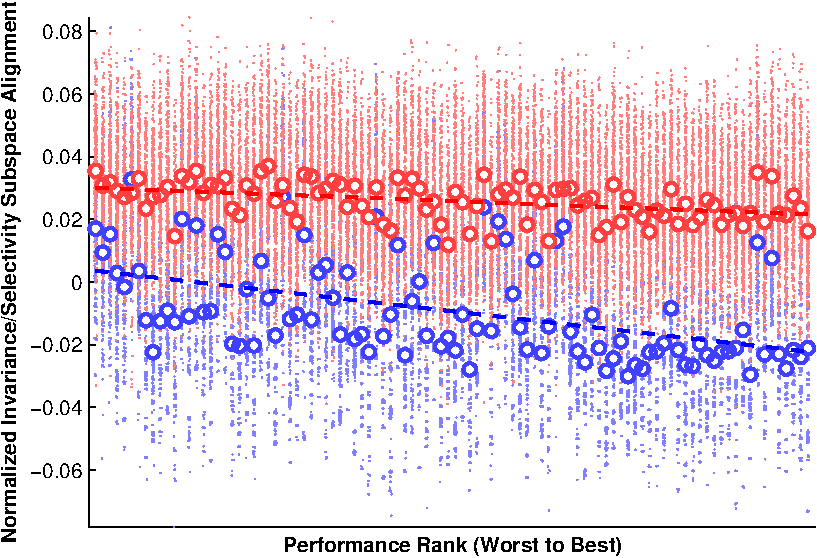
\includegraphics[width=0.6\textwidth]{Figs/e_fig5d.pdf}
\caption{ 
{\bf Invariance and selectivity subspace alignments vs.~performances of deep networks.} Each red distribution from left to right shows the invariance subspace alignments against the task-related stimuli of population representations of a deep network given the 16 reference stimuli. Alignment scores are normalized by subtracting the corresponding reference stimuli's own alignment scores. Performance ranks, instead of performance values, are used for visualization purposes. Means of distributions are plotted as red circles and the linear regression as dashed red line. Blue distributions for selectivity subspace alignments follow the same definitions. Significances of slopes using permutation tests both have $p < 0.001$.}
\label{fig:SFaln}
\end{figure}

\begin{figure}[H]
\centering 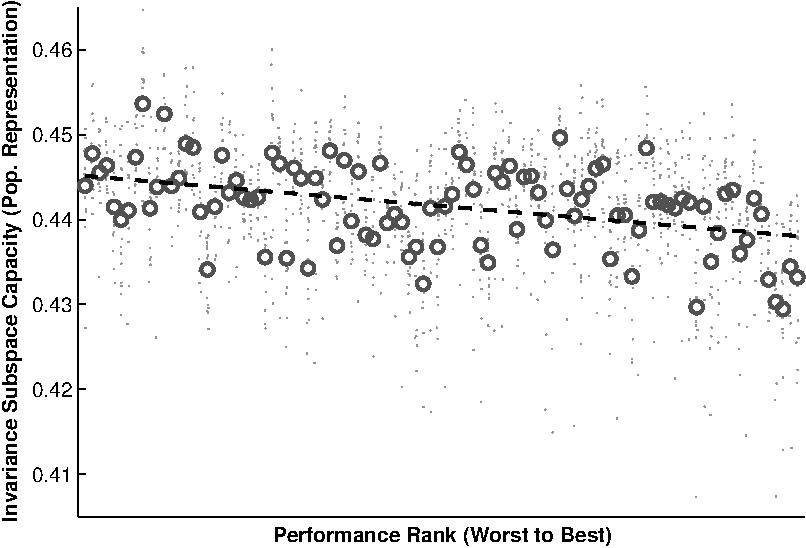
\includegraphics[width=0.6\textwidth]{Figs/e_fig5b.pdf}
\caption{ 
{\bf Invariance subspace capacities vs.~performances of deep networks.} Each distribution from left to right shows the invariance subspace capacities of population representations of a deep network given the 16 reference stimuli. Performance ranks, instead of performance values, are used for visualization purposes. Means of distributions are plotted as gray circles and the linear regression as dashed black line. Significance of slope using permutation test has $p < 0.001$.}
\label{fig:SFinc}
\end{figure}

\begin{figure}[H]
\centering 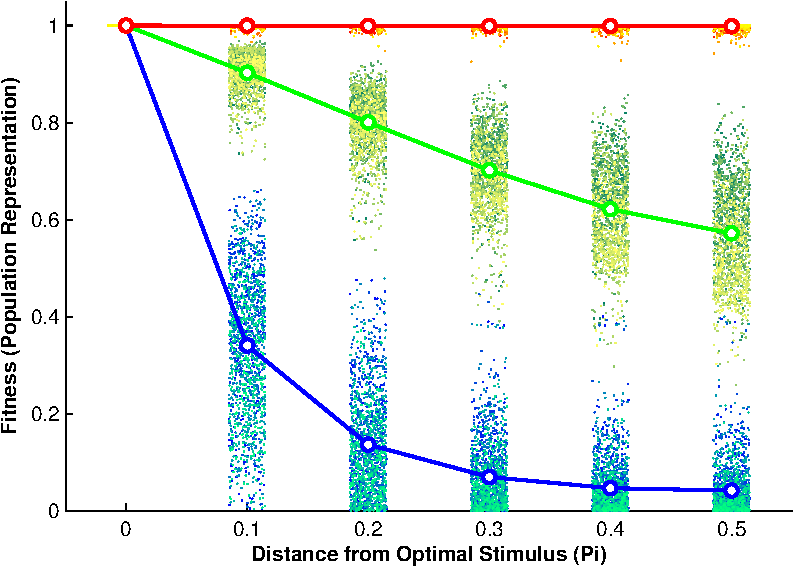
\includegraphics[width=0.6\textwidth]{Figs/e_fig5a.pdf}
\caption{ 
{\bf Fitness-distance diagram of population representations within deep networks.} Red, blue, and green dots indicate results of invariance and selectivity path searches, and random walks, where brighter shades of a color are of better performing networks, and 
darker shades of poor performing networks. Means of results are plotted as solid lines in corresponding colors. As visualized, there is no apparent strong correlations between invariance and selectivity path potentials and performance. Random walk results vs.~performance, on the other hand, has $R^2 = 0.18$ correlation which may arise from the differences in sensitivities to noises, though incorporating it into representation measures does not improve the final multiple correlation.}
\label{fig:SFfda}
\end{figure}

\begin{figure}[H]
\centering 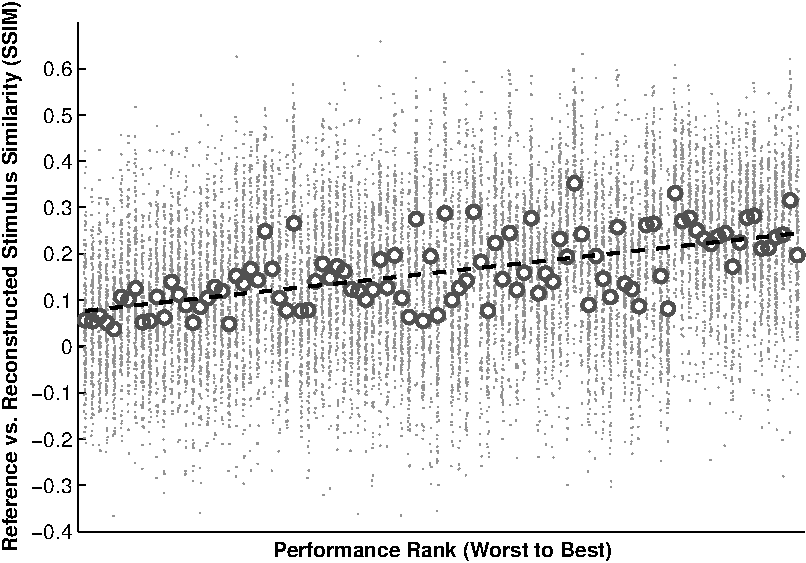
\includegraphics[width=0.6\textwidth]{Figs/e_fig6b.pdf}
\caption{ 
{\bf Encoding specificities vs.~performances of deep networks.} Each distribution from left to right shows the SSIM scores of the reconstructed stimuli of population representations of a deep network against the 16 reference stimuli. Performance ranks, instead of performance values, are used for visualization purposes. Means of distributions are plotted as gray circles and the linear regression as dashed black line. Significance of slope using permutation test has $p < 0.001$.}
\label{fig:SFenc}
\end{figure}